\section{Alternative Experimental Designs}

In this section we return to the nonlinear examples presented in the previous chapter and address the choices made in experimental design.
We demonstrate that the decisions made regarding measurement equipment and/or location have an impact on the reduction of uncertainty and accuracy of the MUD point.

We demonstrate the use of the WME map defined in \eqref{eq:qoi_WME_fixed_data} on a problem incorporating a single stream of time-series data for a first-order ODE problem.

\subsection{ODE Example}
Consider an exponential decay problem with uncertain decay rate:

$$
\begin{cases}
\frac{\partial u}{\partial t} & = \param u(t) \\ u(0) &= 0.75
\end{cases}
$$

The solution is described by
\begin{equation}
  u(t) = u_0\exp(-\param t), \; u_0 = 0.75 ,
\end{equation}
where we consider $t \in [0, 3]$, allowing measurements to begin for $t\geq 1$.
\begin{figure}[htbp]
  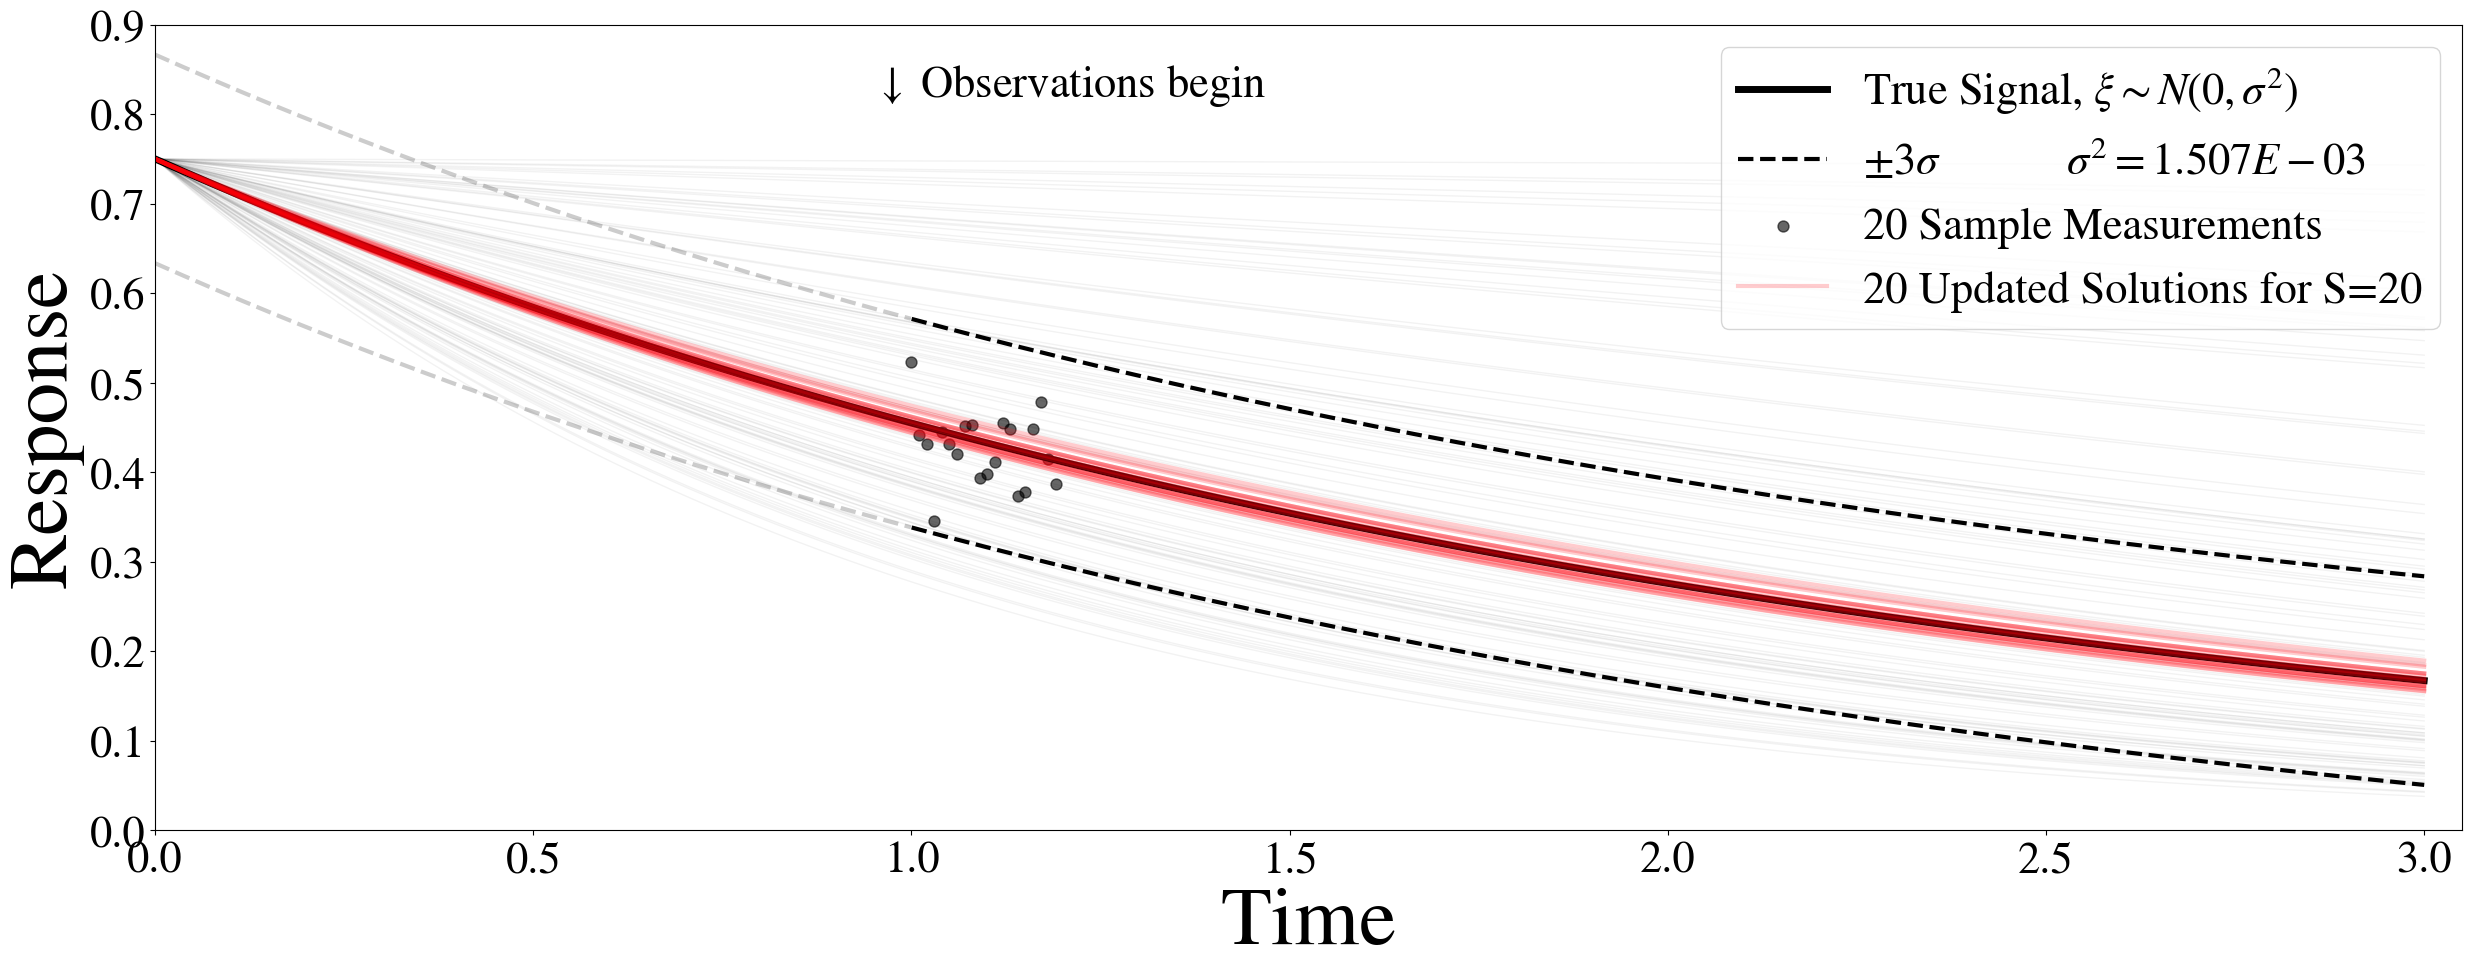
\includegraphics[width=\linewidth]{figures/ode/ode_20_reference_solution}
  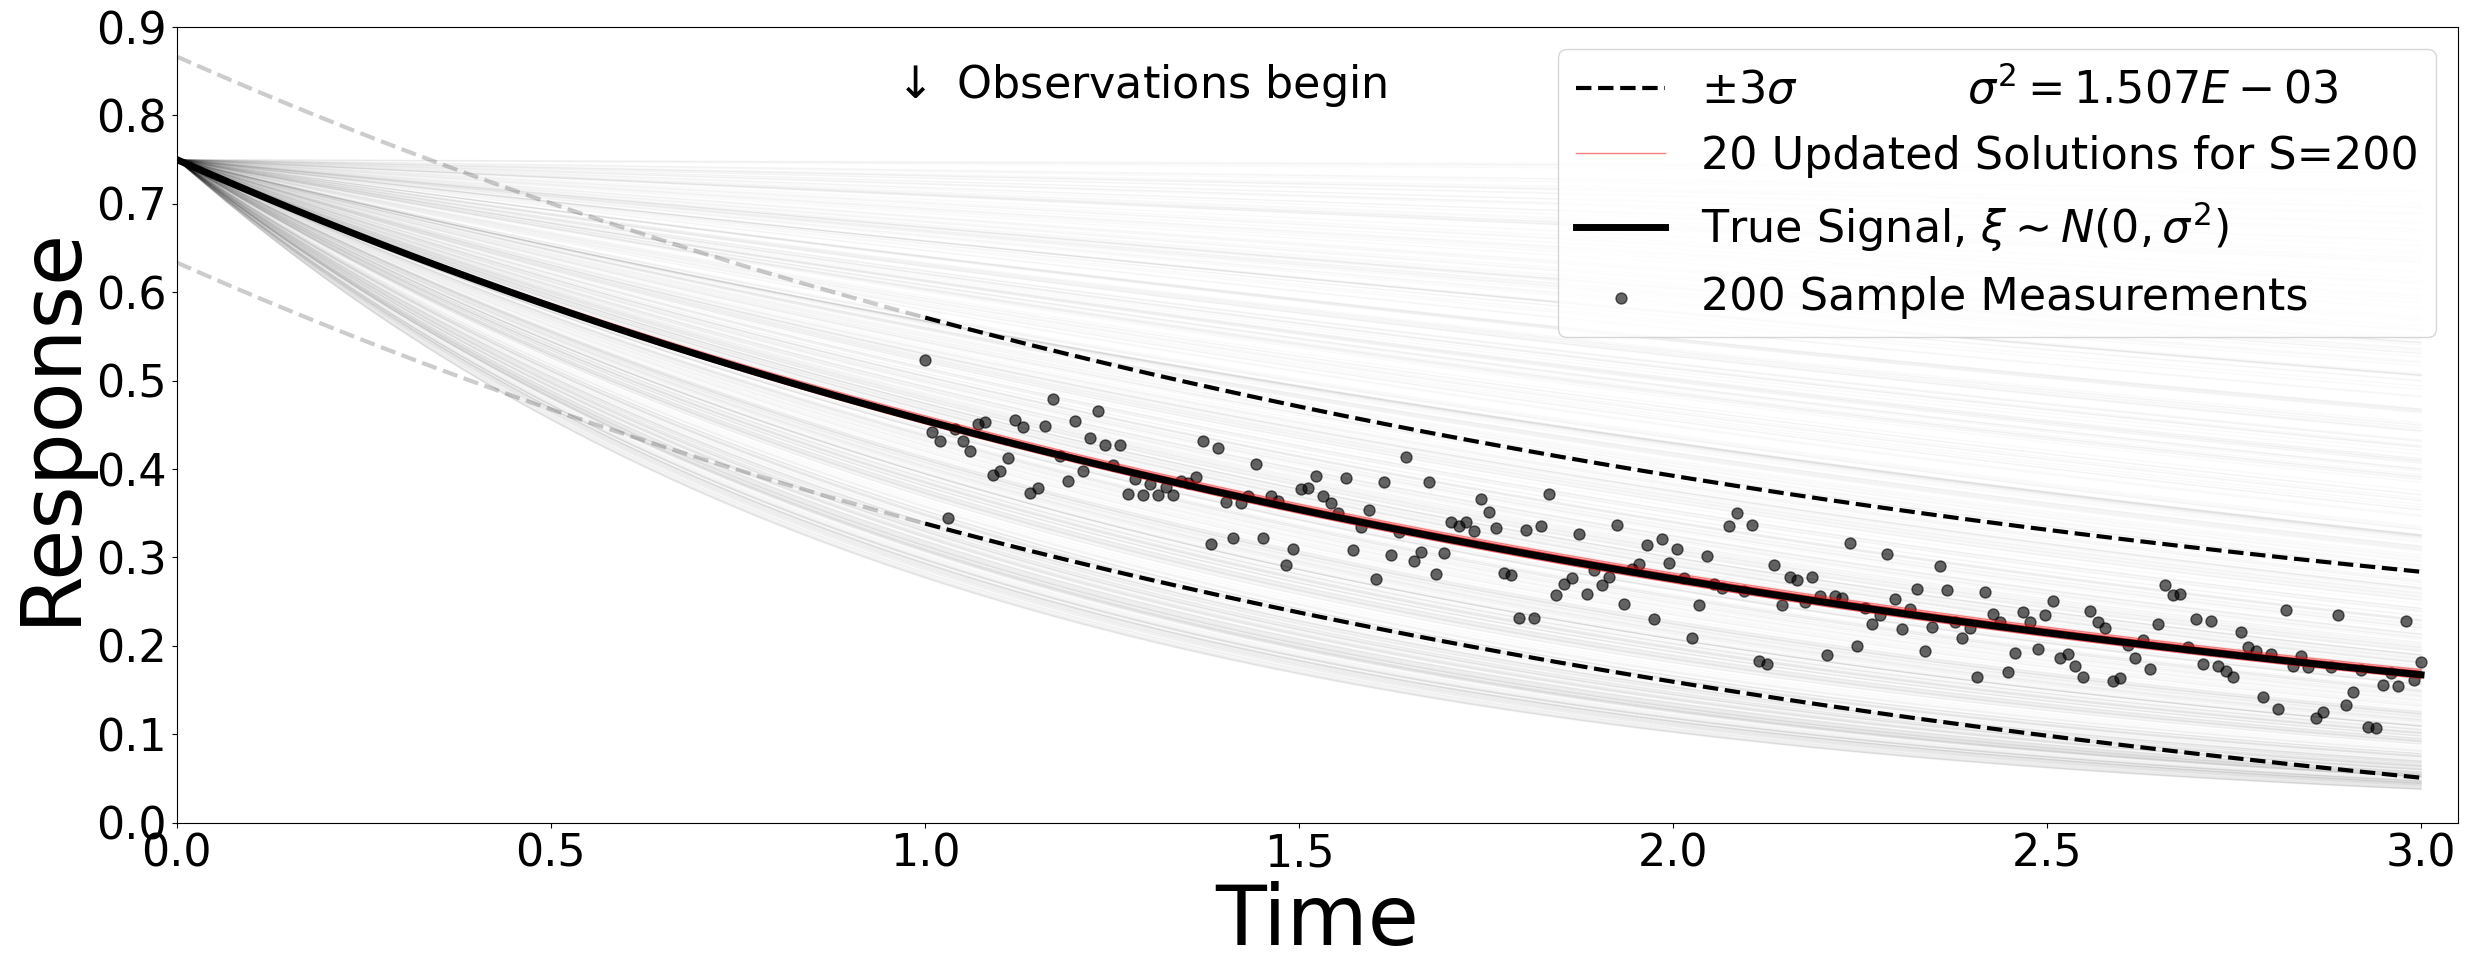
\includegraphics[width=\linewidth]{figures/ode/ode_200_reference_solution}
  \caption{Time series response for exponential decay with markers for the assumed error intervals for observations.
  Measurements are taken over the time interval $(1,3)$.
  Five-hundred draws from $\pi_\text{init}$ are used to generate sample responses and are shown in gray.
  (Top): Twenty updated solution (the results of the repeated trials) for $S=25$ are plotted in blue, and capture the true signal.
  (Bottom): The solution for using all $S=200$ measurements available that were taken over the observation window.
  }
  \label{fig:ode-reference}
\end{figure}

We consider a uniform prior over $\param \in \Lambda = (0, 1)$ to represent our uncertainty about the decay rate.
Measurements are simulated over the interval $t \in [1,3]$ for observations from a $100$Hz sensor, and are perturbed (as outlined in \ref{subsec:example-setup}).
An example of this setup is shown in Figure~\ref{fig:ode-reference}, with the solid line representing the ``true'' signal obtained by evaluating the solution for $\param = 0.5$, and an example of possible measurements shown as perturbed points around it.


\begin{figure}[htbp]
  \centering
  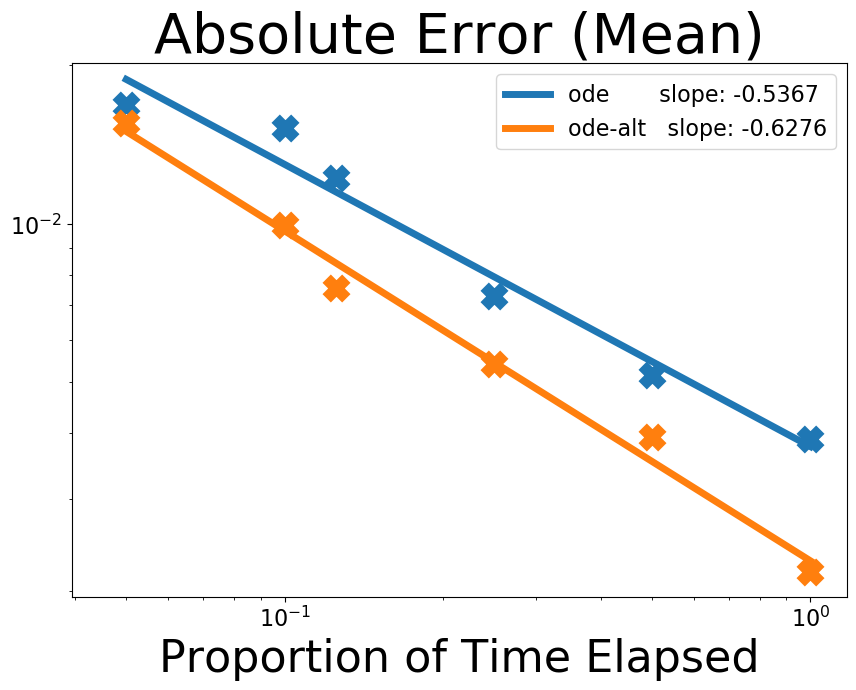
\includegraphics[width=0.475\linewidth]{figures/ode/ode_convergence_mud_obs_mean}
  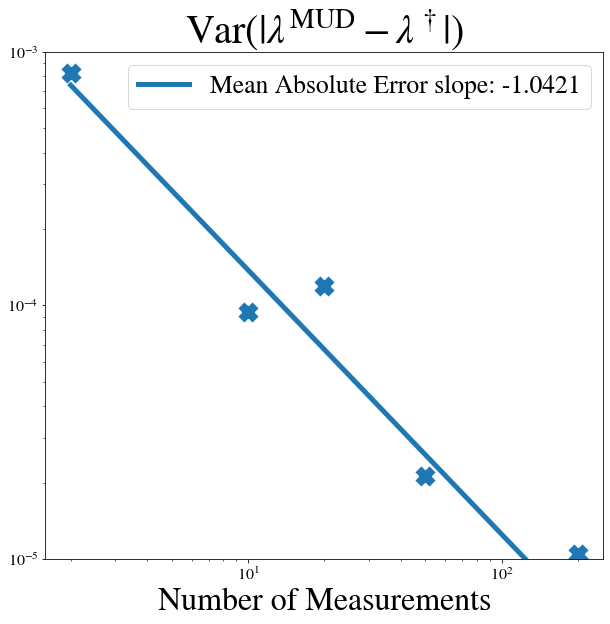
\includegraphics[width=0.475\linewidth]{figures/ode/ode_convergence_mud_obs_var}

  \caption{Convergence of the MUD point given $N=1E4$ model evaluations for increasing numbers of observations for randomly placed sensors.
  Convergence rates are estimated using first-order linear regressions in $\text{log}_{10}$-space.
  $100$Hz equipment demonstrates a reduction of uncertainty and improvement in precision as $S$ increases towards $200$.
  We observe the same rates of convergence for the alternative equipment and note the (slightly) lower overall error for equal numbers of measurements ($S=200$ corresponding to $t\in (1,2)$ in this formulation).
  }
  \label{fig:ode-convergence-obs}
\end{figure}
We sequentially incorporate $S=5, 10, 15, 20, 25, 50, 100, \text{ and } 200$ measurements and study the error in our estimate of $\param_\text{ref}$.
In the top half of Figure~\ref{fig:ode-convergence-obs}, we can observe that as more measurements are incorporated to the solution of the inverse problem, both precision and accuracy are improved.



To achieve higher precision in the estimate of the MUD point, one can use more precise measurement equipment.
Rather than a tolerance of one decimal place, we consider choices of $\tau = 0.1, 0.05, 0.01, 0.005, \text{ and } 0.001$ for $\mathbb{P}( \abs{\xi} < \tau ) = 99\%$ to select our $\sigma$ in our normal additive noise.
In Figure~\ref{fig:ode-convergence-std}, we study the absolute error's mean and variance as our measurement equipment gets more precise.


\begin{figure}[htbp]
  \centering
  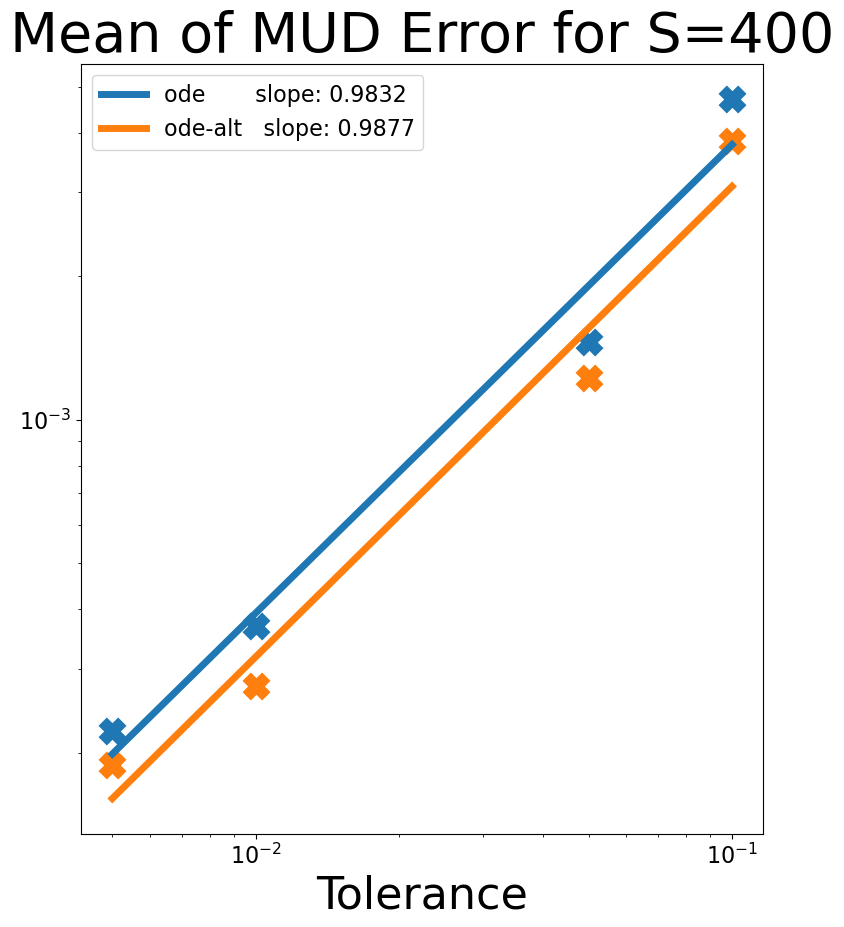
\includegraphics[width=0.475\linewidth]{figures/ode/ode_convergence_mud_std_mean}
  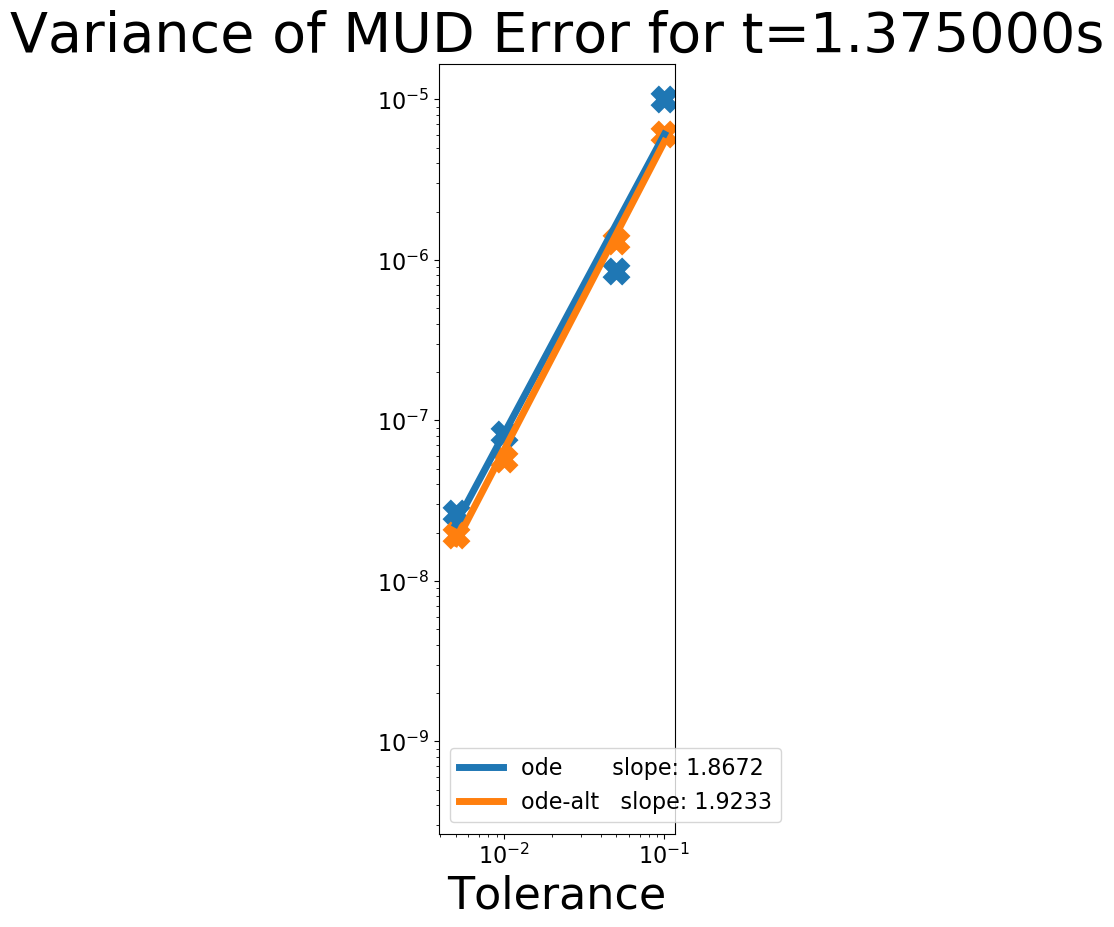
\includegraphics[width=0.475\linewidth]{figures/ode/ode_convergence_mud_std_var}

  \caption{Convergence of the MUD point given $N=1E4$ model evaluations for different precisions of observations for randomly placed sensors, incorporating $S=25$ measurements.
  As more exact measurements are incorporated, the accuracy and precision of the MUD solution improves, convergence rates are estimated with regression, and appear to be unaffected .
  }
  \label{fig:ode-convergence-std}
\end{figure}

TK - say more here.


%%%%%%%%%%%%%%%%%%%%%%%%%%%%%%%%%%%%%%%%%%%%%%%%%%%%%%%%%%%%%%%%%%%%
%%%%%%%%%%%%%%%%%%%%%%%%%%%%%%%%%%%%%%%%%%%%%%%%%%%%%%%%%%%%%%%%%%%%
\subsubsection{Different Measurement Equipment}

We consider the same problem as in the previous section to address the following question: what would happen if our measurement equipment were able to capture twice as many observations?
Instead of using equipment that operates at $100$Hz, we take $200$ measurements every second, resulting in 400 equispaced observations for $t \in (1,3)$.
All other choices involved in the experiment (assumed equipment tolerance, number of trials, parameter samples) are kept the same.

\begin{figure}[htbp]
  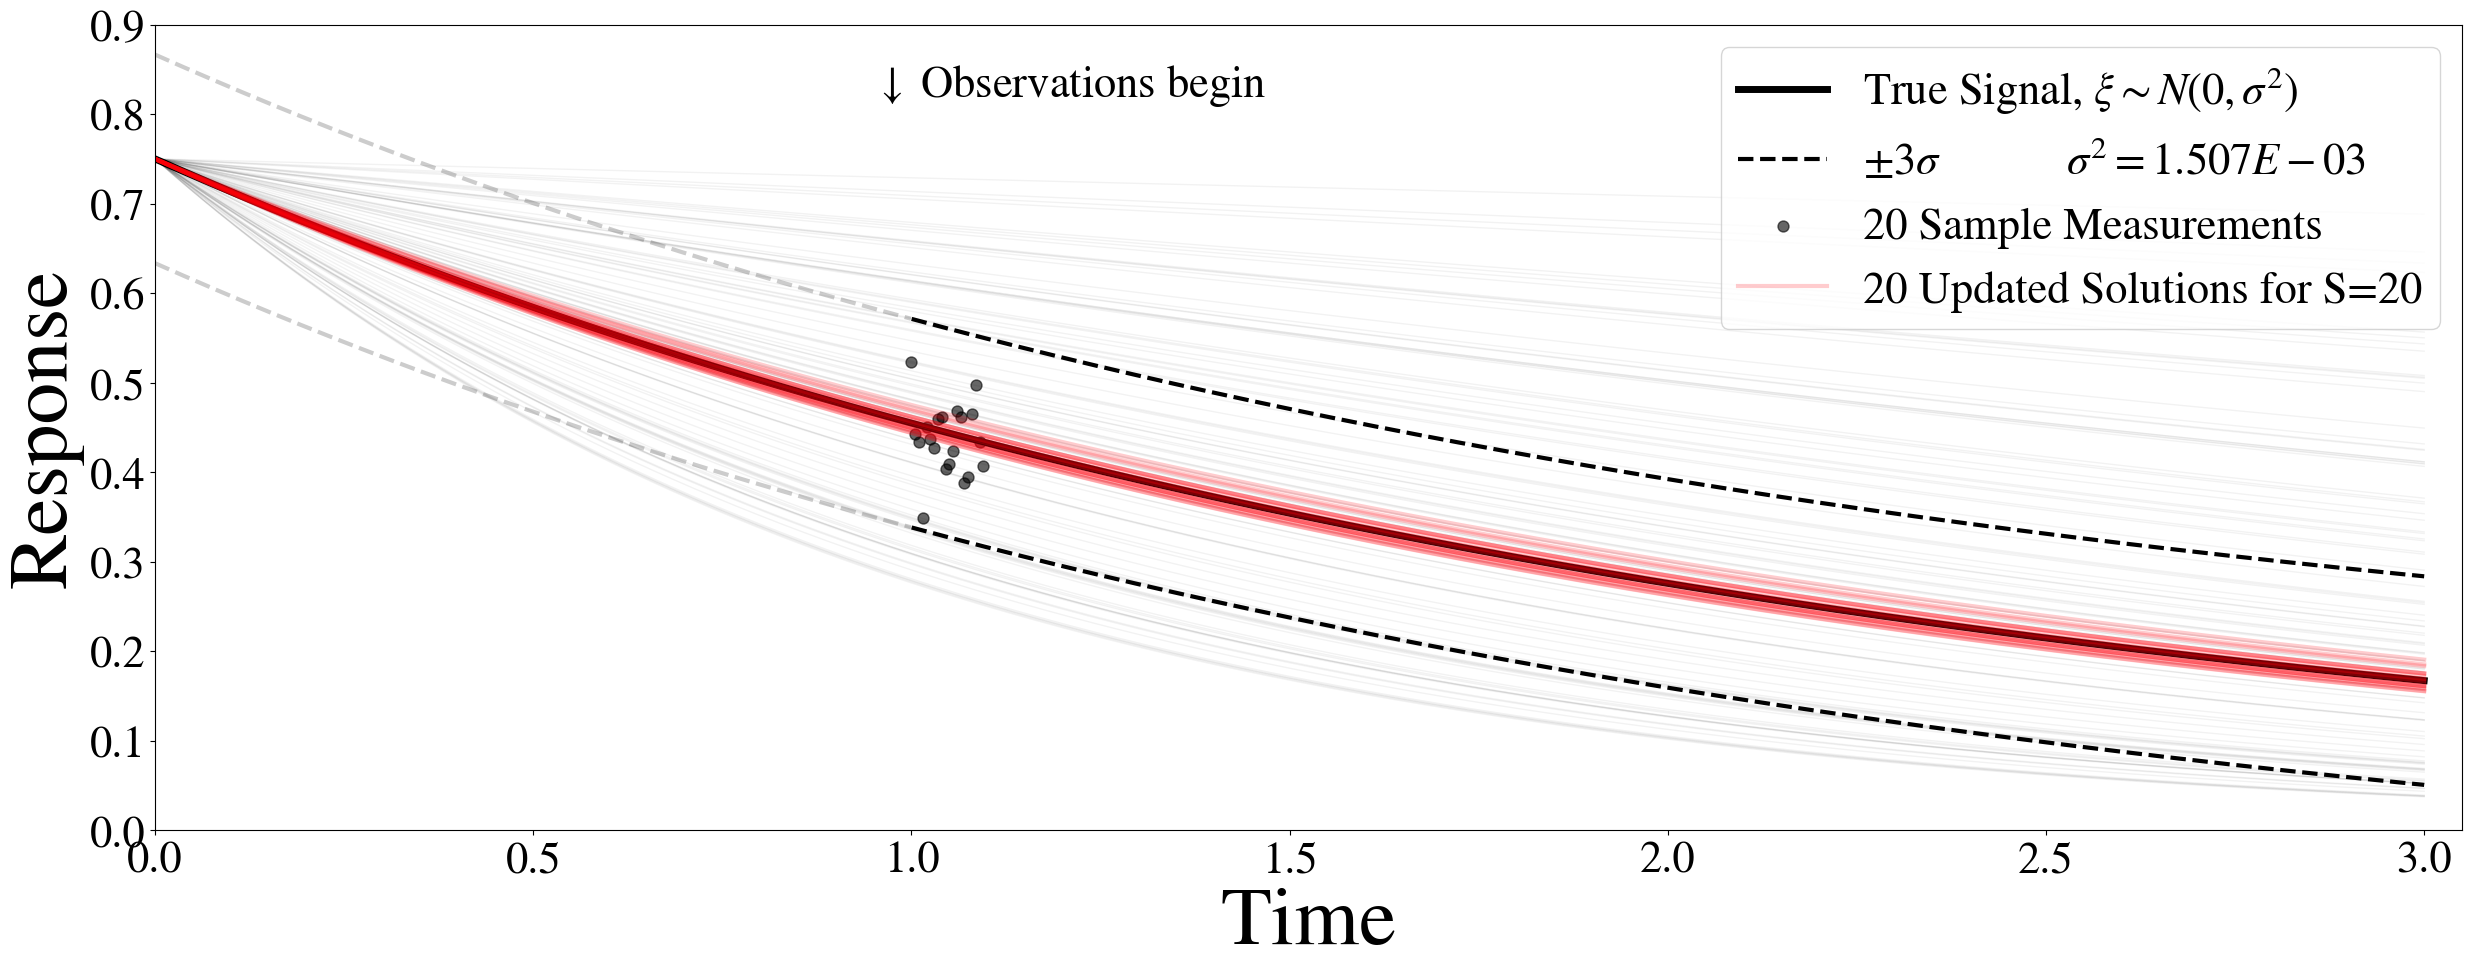
\includegraphics[width=\linewidth]{figures/ode/ode-alt_20_reference_solution}
  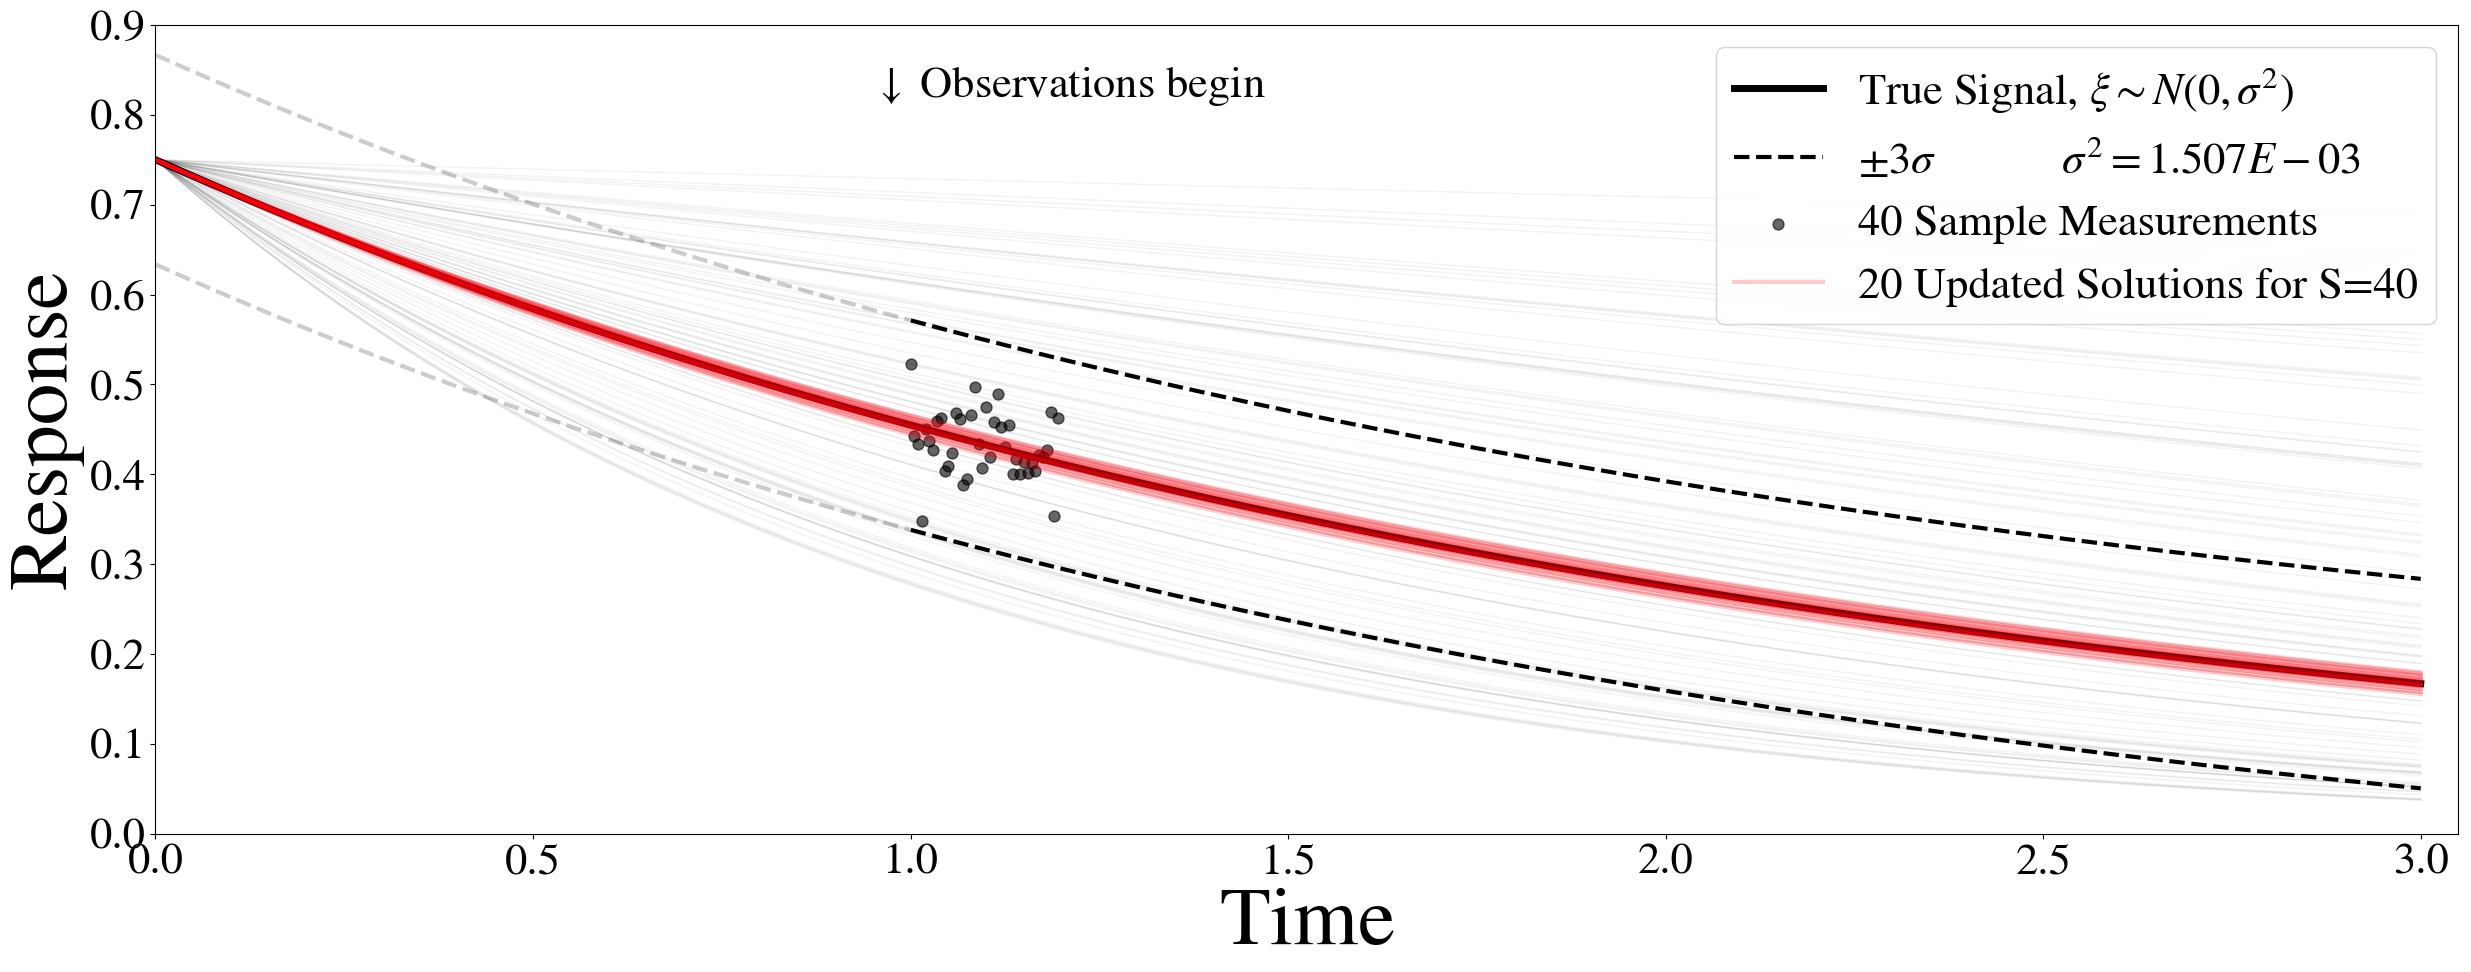
\includegraphics[width=\linewidth]{figures/ode/ode-alt_40_reference_solution}
  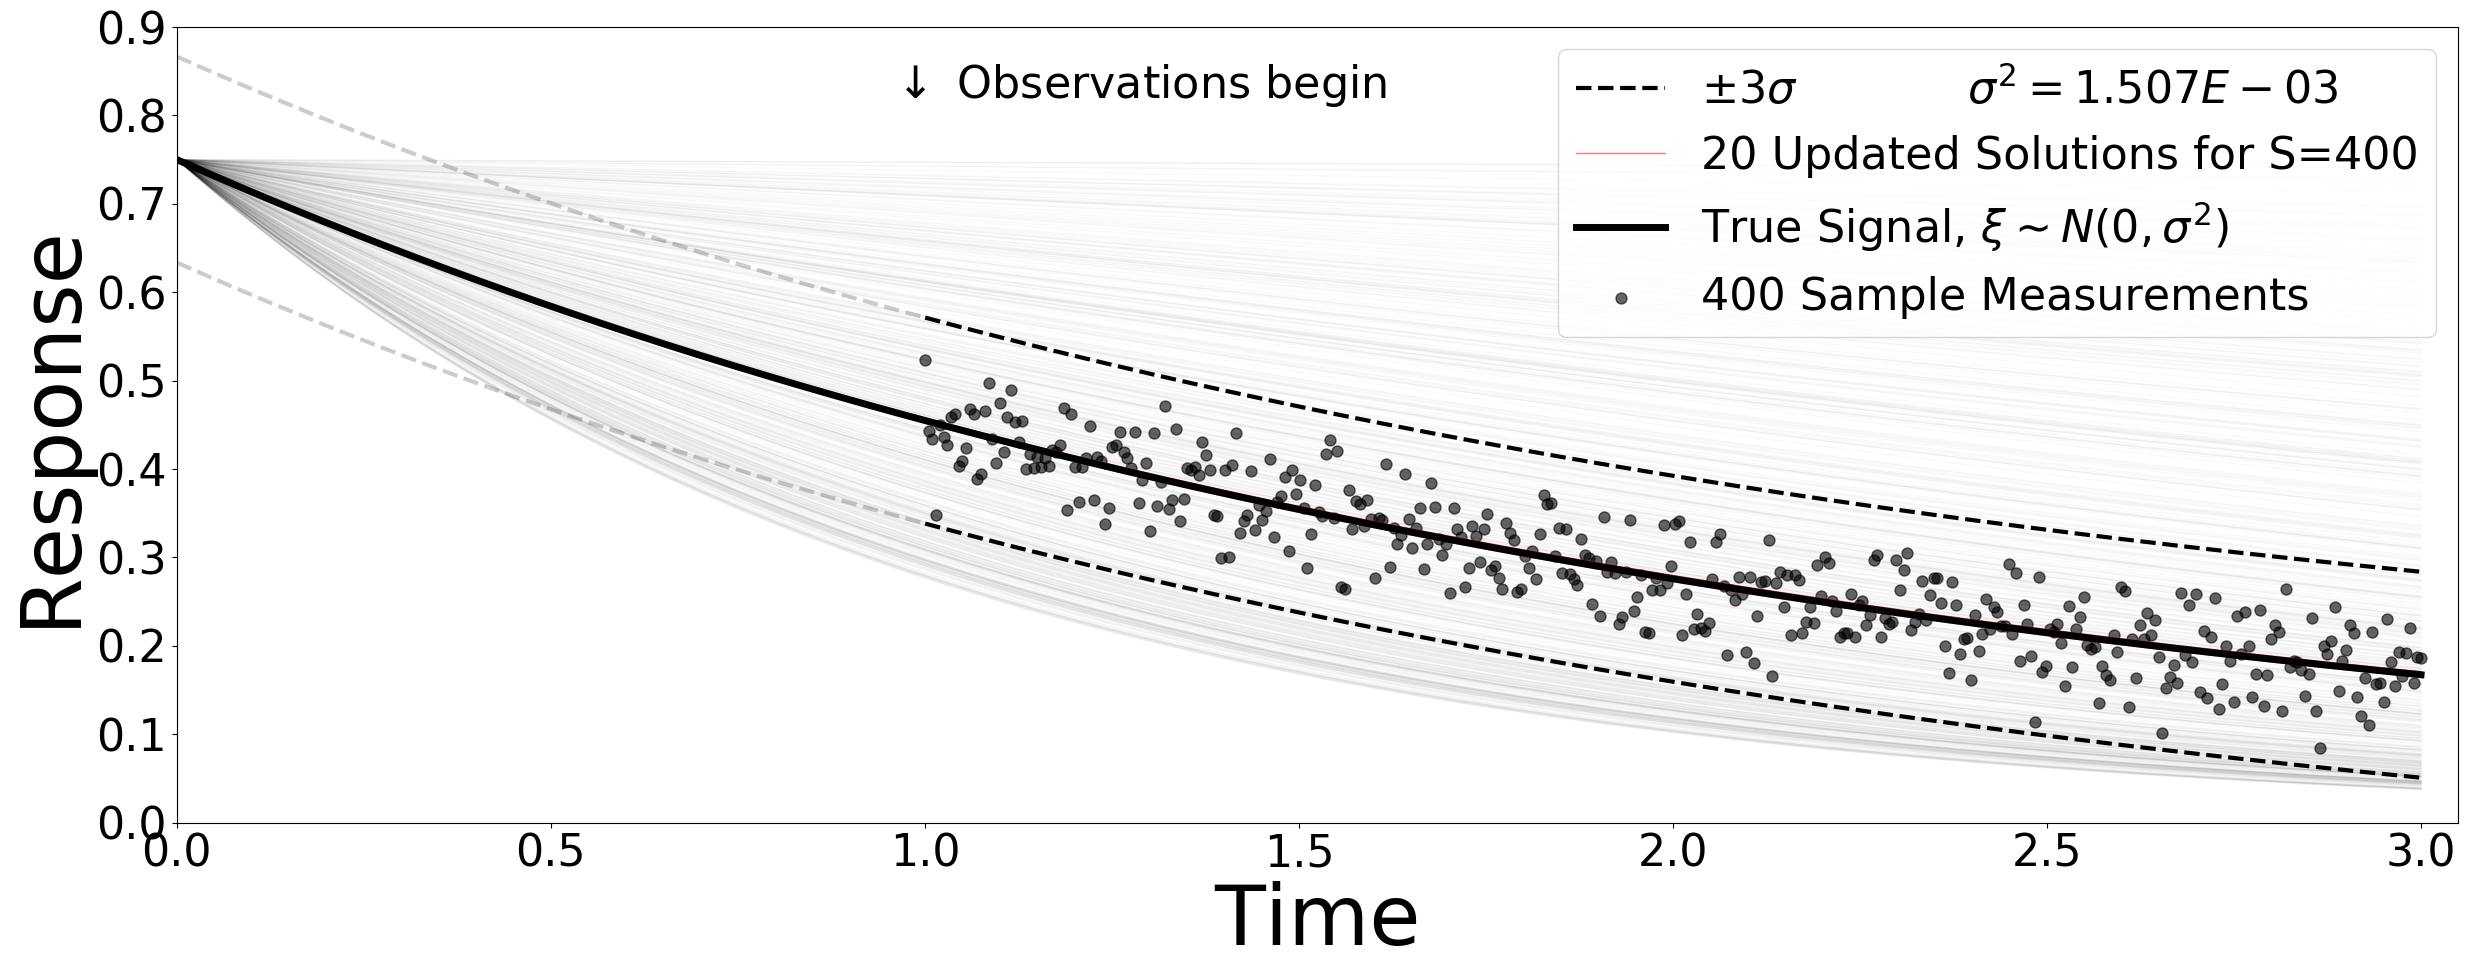
\includegraphics[width=\linewidth]{figures/ode/ode-alt_400_reference_solution}
  \caption{The associated signals for the alternative measurement equipment that operates at twice the frequency.
  The true signal is well-recovered.
  (Top): First twenty-five measurements.
  (Middle): Observations made over the same time interval as in the top half of Figure~\ref{fig:ode-reference}, corresponding to $S=50$.
  (Bottom): The entire observation window is used to solve the problem. Most of the twenty trials appear to identify the same point $\param_i$ ($1\leq i \leq N$), in the sampled parameter set.
  }
  \label{fig:ode-alt-reference}
\end{figure}
First, we note that in Figure~\ref{fig:ode-alt-reference} the predicted signals incorporating the same number of measurements look indistinguishable for $S=25$ compared to those in Figure~\ref{fig:ode-reference}.



We solve the problem for the same choices of $S$ (with the addition of $S=400$, and show the resulting error plots for convergence in the right half of Figures~\ref{fig:ode-convergence-obs} and \ref{fig:ode-convergence-std}.
The convergence rates appear to be the same and reduction in uncertainty is almost negligible.
However, we note that in the alternative setup, for an equal number of measurements, the time elapsed is half of that in the original.
This implies that we can achieve similar results with a shorter observational window by using equipment that allows for faster observations.

We have shown that the Data--Consistent approach to solving parameter identification problems manages to generalize to problems involving time-series data from a single Quantity of Interest.
We now turn our attention to an example where instead of temporal measurements, we incorporate spatial ones to solve another parameter identification problem.
% \vfill
% \pagebreak



%%%%%%%%%%%%%%%%%%%%%%%%%%%%%%%%%%%%%%%%%%%%%%%%%%%%%%%%%%%%%%%%%%%%
%%%%%%%%%%%%%%%%%%%%%%%%%%%%%%%%%%%%%%%%%%%%%%%%%%%%%%%%%%%%%%%%%%%%

%%%%%%%%%%%%%%%%%%%%%%%%%%%%%%%%%%%%%%%%%%%%%%%%%%%%%%%%%%%%%%%%%%%%
%%%%%%%%%%%%%%%%%%%%%%%%%%%%%%%%%%%%%%%%%%%%%%%%%%%%%%%%%%%%%%%%%%%%
\subsection{Elliptic PDE Example}\label{subsec:pde-example}

Consider the following Poisson problem defined on a unit domain:
\begin{equation}\label{eq:pde-equation}
\begin{cases}
\hfill -\nabla \cdot \nabla u &= f \quad\text{on } \Omega \\
\hfill u &= 0 \quad\text{ on } \Gamma_T \cup \Gamma_B \\
\hfill \frac{\partial u}{\partial \mathbf{n}} &= g(x,\param) \quad\text{ on } \Gamma_L \\
\hfill \frac{\partial u}{\partial \mathbf{n}} &= 0 \quad\text{ on } \Gamma_R
\end{cases}
\end{equation}
where $(x_1, x_2) \in \Omega = (0,1)^2$, $\Gamma_T$ is the top, $\Gamma_B$ is the bottom, $\Gamma_L$ and $\Gamma_R$ left and right, respectively.
$\frac{\partial u}{\partial \mathbf{n}}$ denotes the outward normal direction.

\begin{figure}[htbp]
\centering
  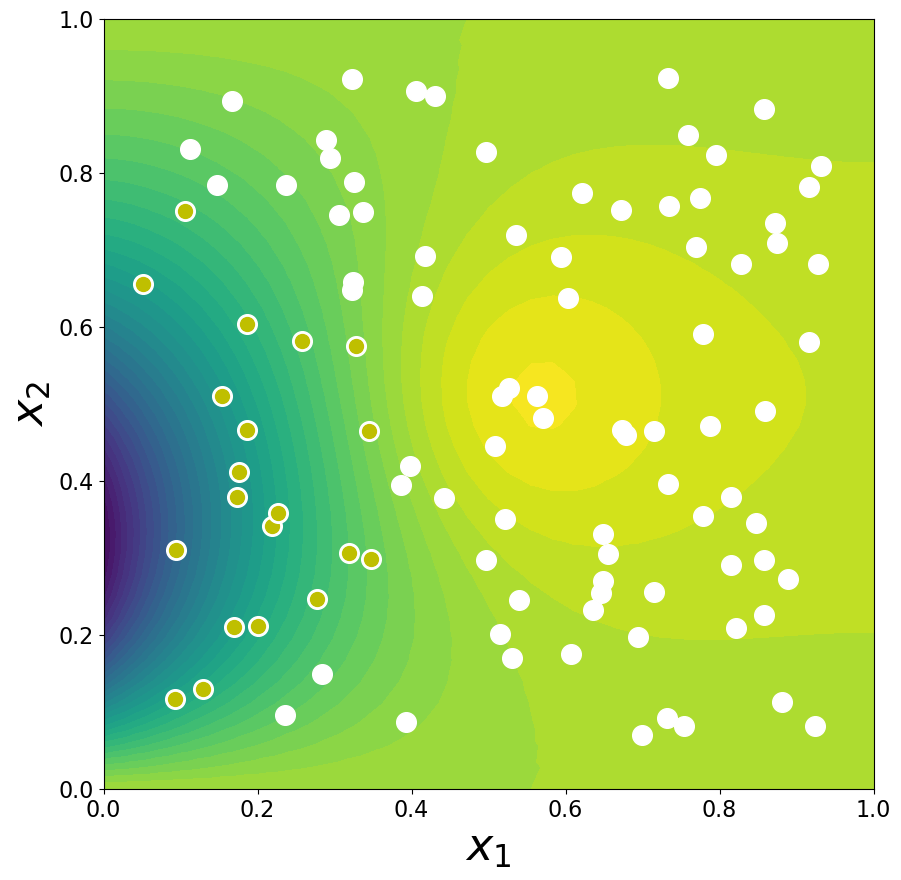
\includegraphics[width=0.475\linewidth]{figures/pde/pde_reference_solution}
  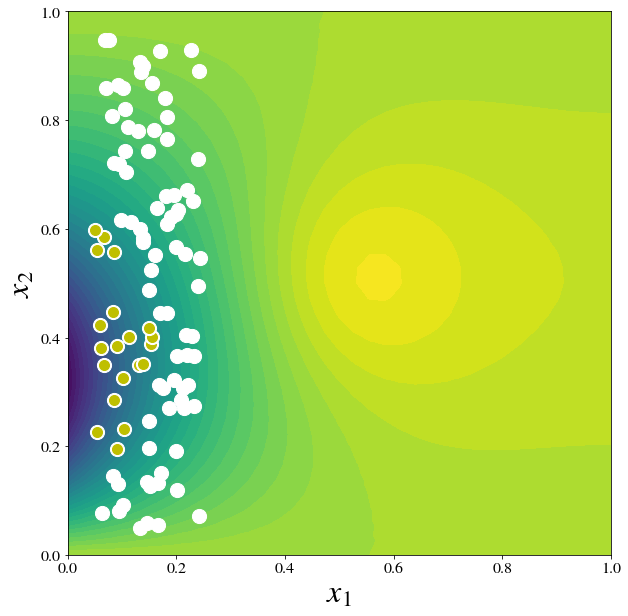
\includegraphics[width=0.475\linewidth]{figures/pde/pde-alt_reference_solution}
\caption{The function response surface for $u$ solving \eqref{eq:pde-equation} with $S=100$ measurement locations highlighted in white.
The twenty most sensitive locations are highlighted in yellow.
(Top): Uninformed sensor placement, where the most sensitive points  appear to cluster around the center of the  left boundary.
This observation is used to inform a better placement.
(Bottom): An alternative random arrangement of $S=100$ measurement locations.
}
\label{fig:pde-ref-solution}
\end{figure}
We select $g=\param \sin(\pi x_2)$, and show the response surface for our given choice of $\param = 3$ in Figure~\ref{fig:pde-ref-solution}.
Our initial density is chosen to be uniform over the interval $\Lambda = (1,5)$.
$f$ is chosen to be $10\exp\{-\frac{(x_1-0.5)^2 + (x_2 - 0.5)^2}{0.02}\}$



One could place a regular grid of sensors in the interior of $\Omega$ to simulate a sensor array of some sort.
However, observe that the response surfaces shown in Figure~\ref{fig:pde-ref-solution} exhibit vertical symmetry about the line $x_1=0.5$ (as a result of our choice of $g$).
We are interested in demonstrating the impact of incorporating more measurements, which poses a problem for this particular experimental design since it will heavily rely on the way in which the sensor grid is indexed.
For example, if the first half of indexed sensors corresponded to the bottom half of $\Omega$, the incorporation of the second half will be equivalent to having repeated observations.
Moreover, since the left-side of $\Omega$ is more sensitive to changes in $\param$ than the right, indexing in a serpentine manner will lead to sharper declines in uncertainty whenever a sensor from a different row gets incorporated.
To avoid these problems, we instead simulate the sensors as being placed randomly in the interior so that index-dependence becomes irrelevant and  probability theory ensures the lack of truly redundant measurement locations.

%%%%%%%%%%%%%%%%%%%%%%%%%%%%%%%%%%%%%%%%%%%%%%%%%%%%%%%%%%%%%%%%%%%%
%%%%%%%%%%%%%%%%%%%%%%%%%%%%%%%%%%%%%%%%%%%%%%%%%%%%%%%%%%%%%%%%%%%%
\subsubsection{Uninformed Sensor Placement}

We consider a selection of $S=1000$ measurement locations in the interior of the response surface chosen by sampling a uniform density over the set $(0.05, 0.95)^2 \subset \Omega$.
In Figure~\ref{fig:pde-sensitivity}, we plot the data generated by each simulated sensor location, and observe that some measurements are more sensitive in others.
The majority of measurements exhibit almost no sensitivity to changes in $\param$, visually represented by near-horizontal lines.
However, some of the sensors have steep slopes, indicating higher sensitivity to the unknown parameter.
To generate convergence plots, we use all thousand available measurements but solve the problem repeatedly for $S = 5, 10, 15, 20, 25, 50, 100, 250, 500, \text{ and } 1000$.


\begin{figure}[htbp]
\centering
  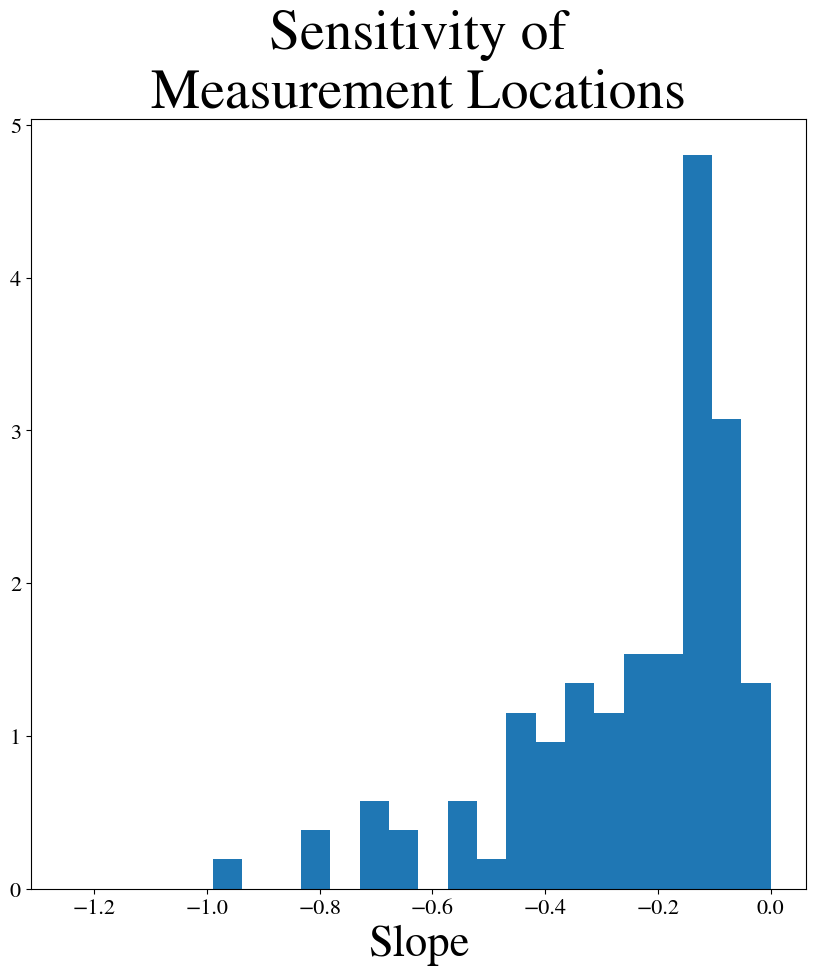
\includegraphics[width=0.35\linewidth]{figures/pde/pde_sensitivity_qoi}
  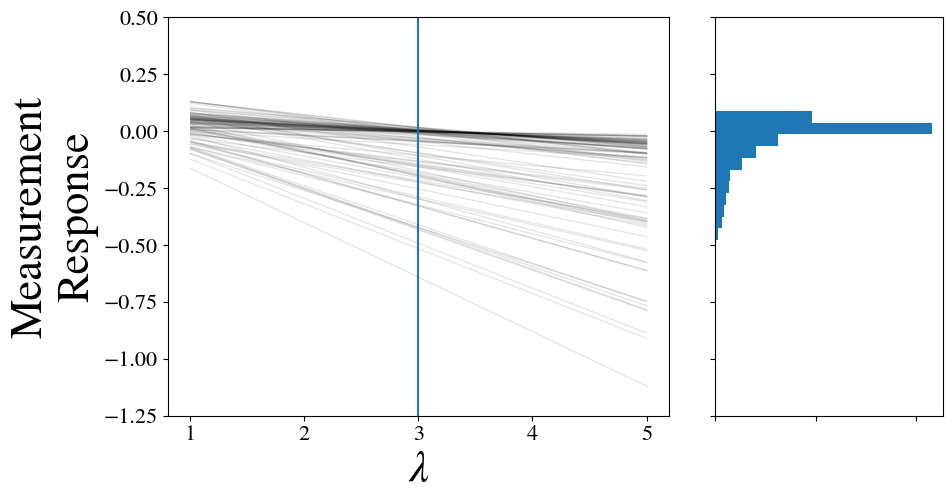
\includegraphics[width=0.6\linewidth]{figures/pde/pde_qoi_response}
  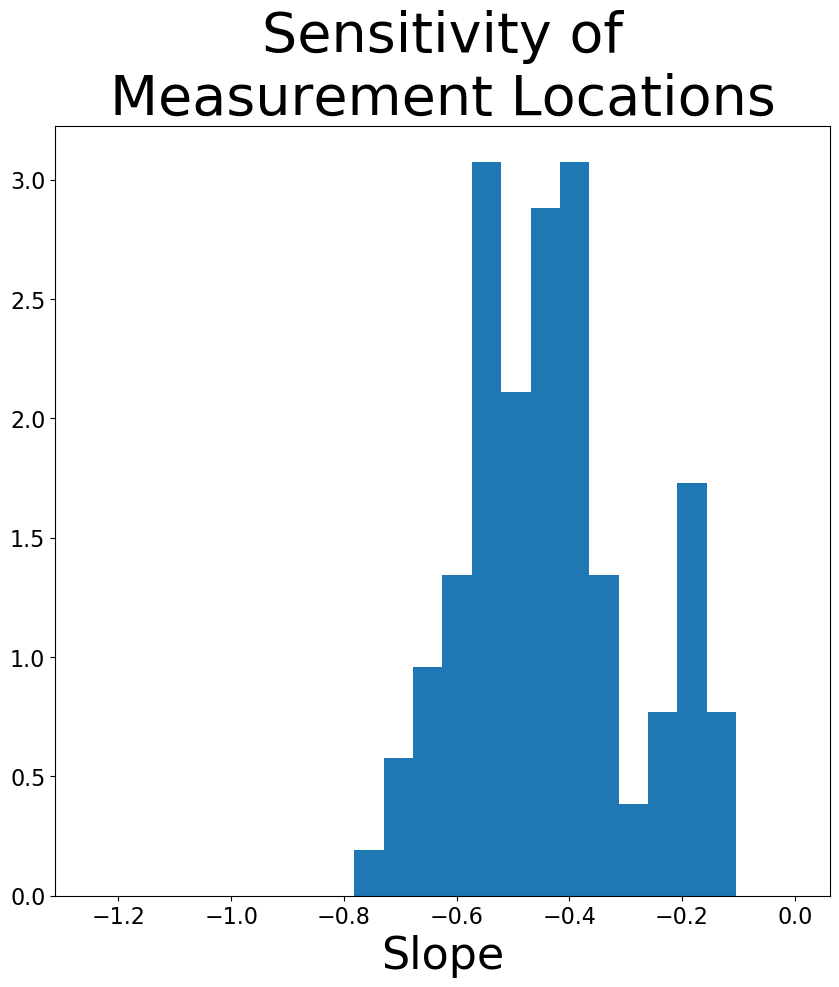
\includegraphics[width=0.35\linewidth]{figures/pde/pde-alt_sensitivity_qoi}
  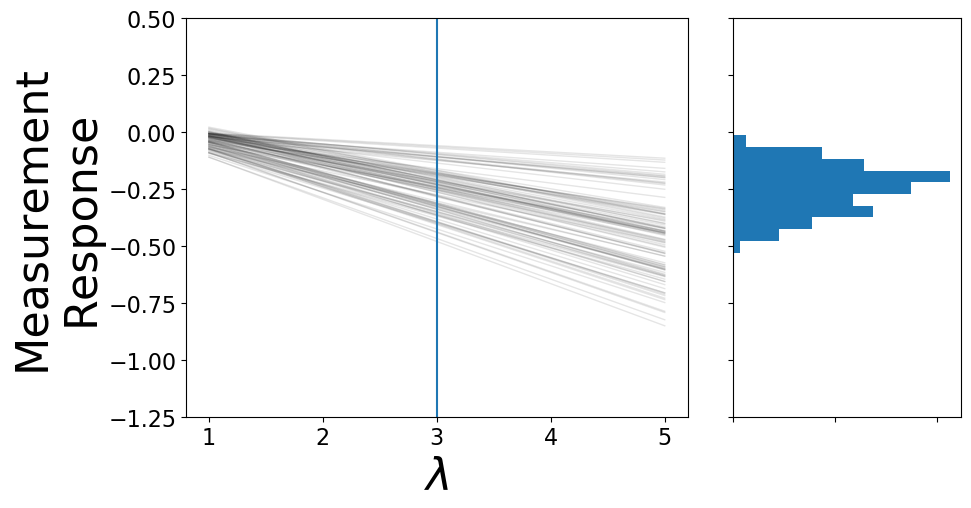
\includegraphics[width=0.6\linewidth]{figures/pde/pde-alt_qoi_response}
  \caption{We plot the values of the response surface evaluated at all $S=1000$ random measurement locations.
  The histogram depicts the measurement values of the response surface evaluated at the true parameter value $\param_\text{ref}=3$.
  (Left): Sensitivity of measurements as a function of $\param$, the scaling for the left boundary condition function.
  (Right): Since the response at each measurement location is linear with respect to $\param$, we compute the slopes for all $S=1000$ sensors and show the associated histogram.
  (Top): Uninformed sensor placement. Observe that most locations are insensitive to changes in $\param$. The ratio of most to least sensitive slopes exceeds 50.
  (Bottom): Informed sensor placement. The informed sensors have much less variability in their respective sensitivities (ratio closer to 10).
  }
\label{fig:pde-sensitivity}
\end{figure}



We are interested in knowing how the uncertainty around the parameter estimate (the MUD point) changes as we incorporate more (noisy) data.
Consider the plots in the left-half of Figure~\ref{fig:pde-convergence-obs}, which demonstrates the impact of increasing $S$ on our ability to resolve $\param_\text{ref}$.


\begin{figure}[htbp]
  \centering
  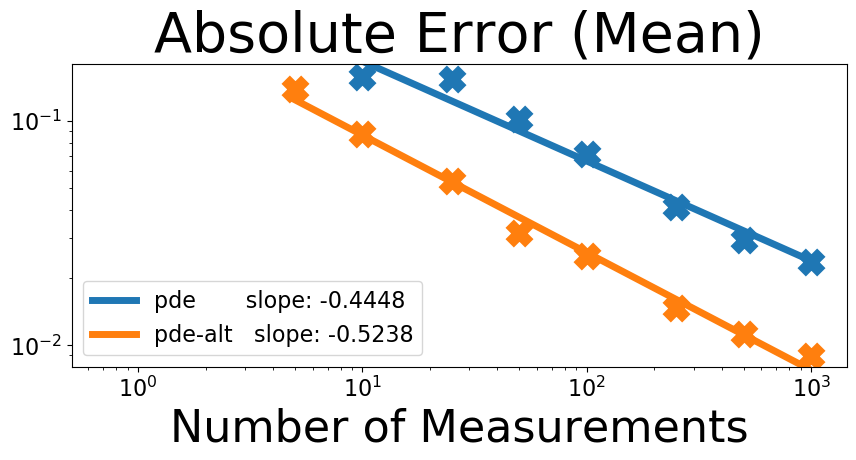
\includegraphics[width=0.475\linewidth]{figures/pde/pde_convergence_mud_obs_mean}
  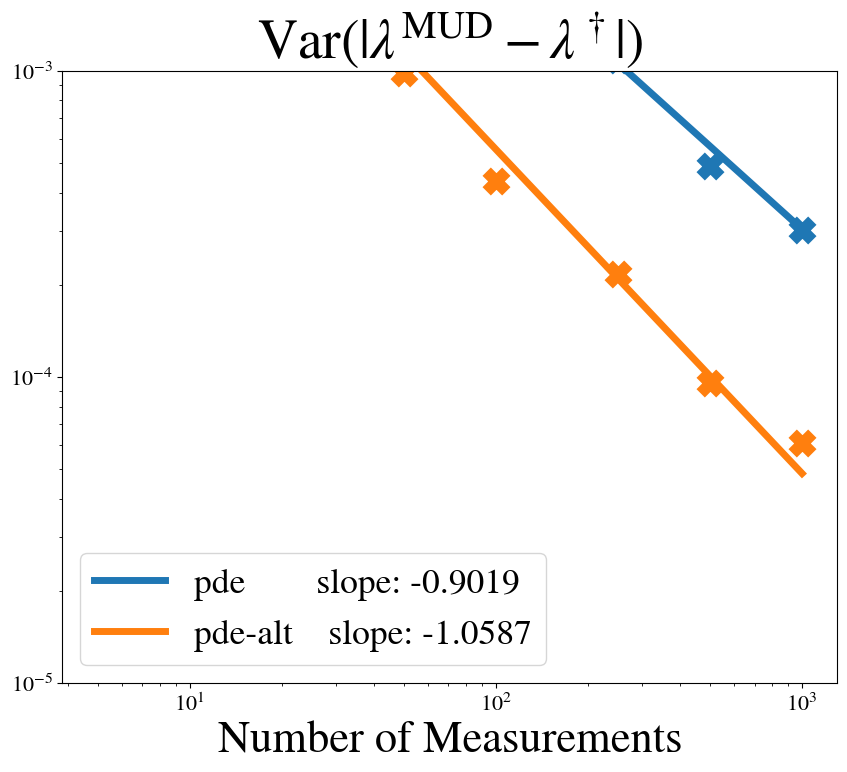
\includegraphics[width=0.475\linewidth]{figures/pde/pde_convergence_mud_obs_var}
  \caption{Convergence of the MUD point (given $N=1E4$ model evaluations) for increasing numbers of observations for randomly placed sensors.
  We observe similar rates of convergence for both arrangements of measurement locations, with a marked improvement in both accuracy and precision when an informed placement is used.
  }
  \label{fig:pde-convergence-obs}
\end{figure}


Similar to \ref{fig:ode-convergence-std}, we demonstrate that using more sensitive measurement equipment improves the estimation of the MUD point.
Again we consider choices of standard deviation associated with $\tau = 0.1, 0.05, 0.01, 0.005, \text{ and } 0.001$ for $\mathbb{P}( \abs{\xi} < \tau ) = 99\%$
In Figure~\ref{fig:pde-convergence-std}, we study the impact of more precise measurement equipment on the absolute error's mean and variance.

\begin{figure}[htbp]
  \centering
  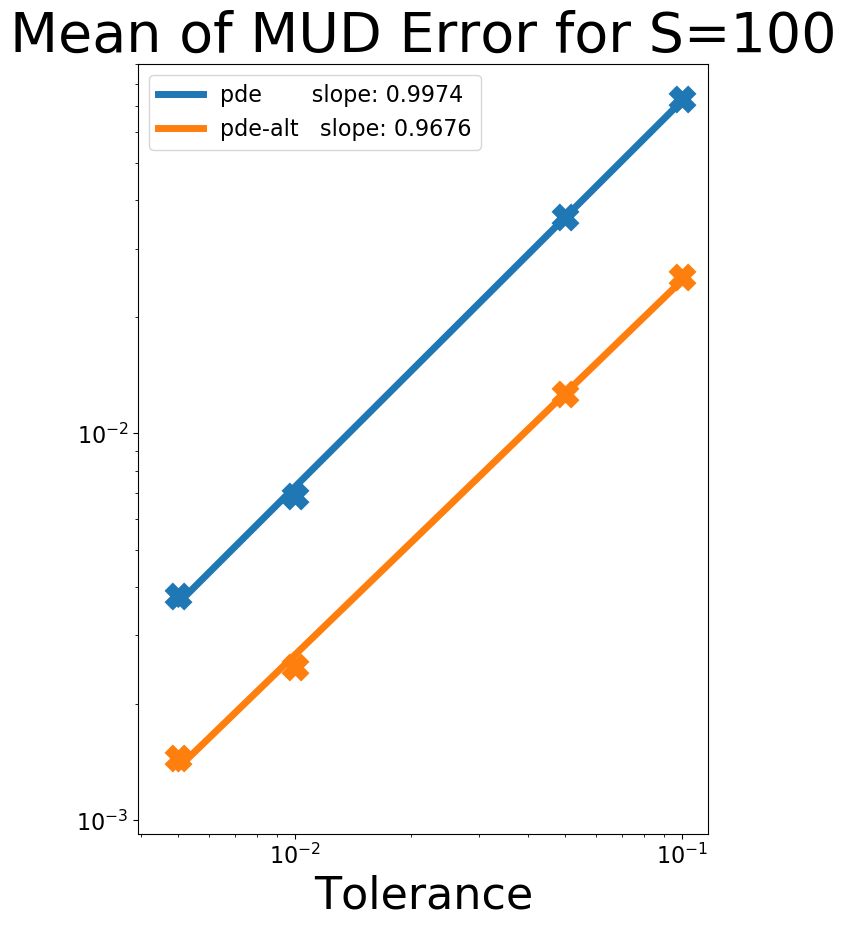
\includegraphics[width=0.475\linewidth]{figures/pde/pde_convergence_mud_std_mean}
  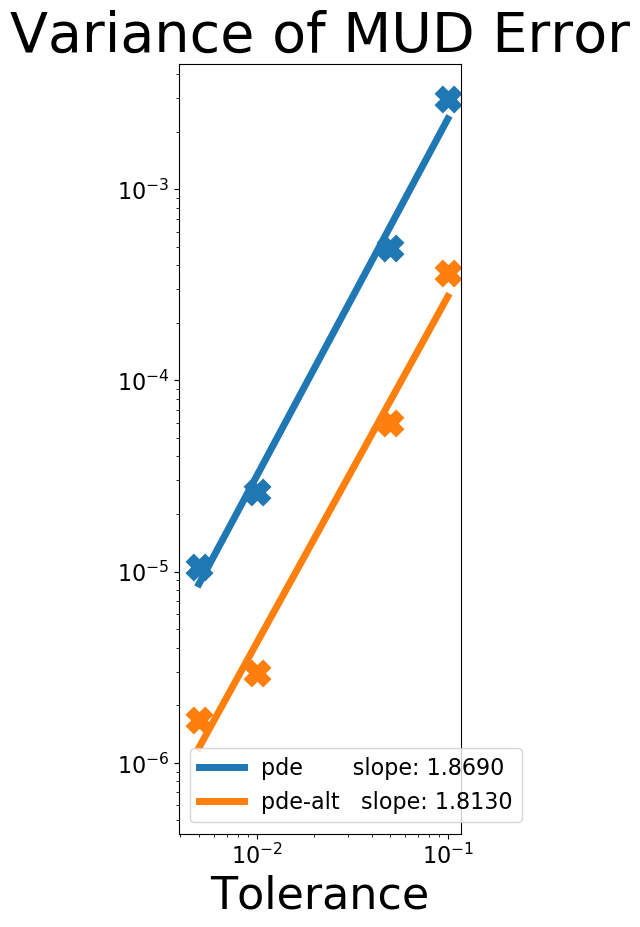
\includegraphics[width=0.475\linewidth]{figures/pde/pde_convergence_mud_std_var}
  \caption{Convergence of the MUD point given $N=1E4$ model evaluations for different measurement precisions for randomly placed sensors, incorporating $S=100$ measurements.
  We note that the convergence rates are the same but the overall accuracy and precision improve when sensors are placed in regions of $u$ that exhibit higher sensitivity to changes in $\param$.
  }
  \label{fig:pde-convergence-std}
\end{figure}


These results demonstrate that even randomly placed sensors in the interior of $\Omega$ are suitable for parameter estimation.
Figure~\ref{fig:pde-ref-solution} shows the twenty most sensitive sensors appear by the left boundary of the domain; choosing sensors more carefully using this information could lead to improved accuracy with fewer sensors.
Let us turn our attention to incroporating this observation into our experimental design chocies.

\subsubsection{Informed Sensor Placement}
Instead of placing sensors throughout the square interior of $\Omega$ given by $(0.05, 0.95)^2$, we briefly consider how the convergence results would change if the subdomain for sensors was better chosen to be near the left boundary.
Furthermore, the response surface exhibits horizontal symmetry, so we restrict locations to the bottom half of $\Omega$.
We perform the same experiment for sensors placed in $(0.05, 0.25)\times(0.05, 0.5)$ and show the results in

We demonstrate the sensitivities of each sensor in the right half of Figure~\ref{fig:pde-sensitivity}, and note that there are fewer sensors twhich exhibit low sensitivity to changes in $\param$.
It appears in the right half of Figure~\ref{fig:pde-convergence-obs}, that two decimal places of accuracy can be achieved with approximately $250$ samples instead of the $1000$ required in the left-half.


TK - Closing statements about optimal experimental design being out of the scope of this work, but how this was an interesting thing to observe.

%%%%%%%%%%%%%%%%%%%%%%%%%%%%%%%%%%%%%%%%%%%%%%%%%%%%%%%%%%%%%%%%%%%%
%%%%%%%%%%%%%%%%%%%%%%%%%%%%%%%%%%%%%%%%%%%%%%%%%%%%%%%%%%%%%%%%%%%%

%%%%%%%%%%%%%%%%%%%%%%%%%%%%%%%%%%%%%%%%%%%%%%%%%%%%%%%%%%%%%%%%%%%%
%%%%%%%%%%%%%%%%%%%%%%%%%%%%%%%%%%%%%%%%%%%%%%%%%%%%%%%%%%%%%%%%%%%%
\subsection{Concluding Remarks for Examples}

As these examples demonstrate, Data--Consistent Inversion can be used for parameter identification as a viable alternative to existing methods.
These problems have involved one-dimensional input and output spaces, and so the resulting problems were not necessarily ones that would benefit from regularization.

We point out that in the framework of collapsing available observations of data leaves the output space as scalar-valued.
As the number of parameters grows, this output dimension effectively stays fixed.
This is particularly when the DCI approach becomes advantageous.
One can incorporate a much wider variety of prior beliefs about the relative likelihoods of parameters before data is collected without compromising predictive error.
The DCI approach guarantees that the functional defined (for us, the weighted mean error) will remain accurate in spite of any encoded assumptions that are somehow at odds with data that is subsequently collected.

%%%%%%%%%%%%%%%%%%%%%%%%%%%%%%%%%%%%%%%%%%%%%%%%%%%%%%%%%%%%%%%%%%%%
%%%%%%%%%%%%%%%%%%%%%%%%%%%%%%%%%%%%%%%%%%%%%%%%%%%%%%%%%%%%%%%%%%%%
